\chapter{Implementation}
\label{cha:implementation}

This section describes the actual implementation of the system, how it implements the different functionalities specified in previous sections and how these work together in order to realize the whole system. The different components of the system have been implemented independently with consultation among implementers and interface definitions during the development process, hence each component of the system is provided with its own dedicated section describing its implementation. Before the actual implementation is going to be put forward it is important to revisit the problem that the implementation shall cover and that is a "Maritime container IoT based monitoring system" capable of monitoring status and generating alarms for maritime containers while storing the alarms for historical purposes and also providing mobile interface to field technicians in order to monitor and resolve alarms. The complete system (including components and sub components) and its various interactions can be visualized on the high level architectural diagram:

\bigskip
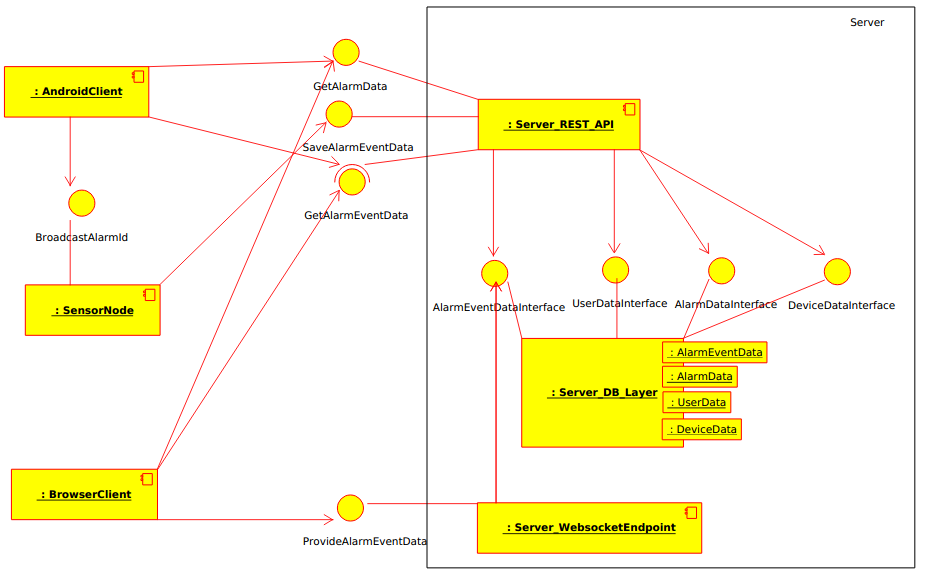
\includegraphics[scale=0.5]{gfx/Architecture}
\smallskip

\section {Central server}
\label {sec:implserver}

This section shows the implementation of the central server component. This component have been developed using Node.js and SQLite. The IDE used to develop the application was primarily JetBrains WebStorm and Microsoft (MS) Visual Studio. This component consists of several cooperating subcomponents, namely:
\begin{enumerate}
	\item REST API component
	\item Websocket component
	\item Web application hosting component
	\item Database layer component following the repository layer (partly)
	\item Database creation scripts
\end{enumerate}

\smallskip
The central server application is structured into several javascript (.js) files in order to provide separation of concern. The .js files in the solution (solution is to be understood as collection of .js files following a specific structure and not neccessarily as MS Visual Studio solution) are: \newline
\begin{enumerate}
	\item Database entity model files
\begin{itemize}
	\item Alarm.js
	\item AlarmEvent.js
	\item AlarmEventResolution.js
	\item Devices.js
	\item Users.js
	\item index.js
\end{itemize}
\item app.js
\item DataAccessLayer.js
\item globals.js
\item packages.json
\end{enumerate}

\smallskip
Most of the implementation of web communication is present directly in the app.js file, while model files and DataAccessLayer.js files represent the database access pattern. The packages.json files specifies which packages should be installed by npm. While the model files represent the database entities (except for the index.js file), the other files deserve more thorough description (due to them containing the whole application logic). One noteworthy mention from module files is that the timestamp are modelled as String datatype due to SQLite not supporting native Timestamp datatype.
\smallskip

\textbf{index.js:} \newline
The file specifies settings for the ORM necessary to work with the SQLite database as well as defines relations between database entities. It follows model loading pattern reccommended for working with separate database entity files by Sequelize.js contributors -> using foreach loop to load database entities based on the filename.

\smallskip
\textbf{app.js:} \newline
The fille that is the entry point to the application. It specifies the whole REST API that the application exposes, WebSocket endpoint exposed by the application and sets up the server (HTTP and WebSocket server). It handles the calls to the database layer based on the calls to the REST API. It uses the DataAccessLayer.js to achieve the database connectivity and globals.js where port numbers are specified for REST API and WebSocket endpoint.

\smallskip
\textbf{DataAccessLayer.js:} \newline
The file specifies database operations used by the application. Unlike the repository pattern it specifies operations for database entities in a single file. The reson for this is rather pragmatic and that is that splitting Sequelize operations and database entities is rather tedious task and no clear pattern for doing this is currently reccommended. Due to this the compromise has been chosen where the database entities each get their own file, while the operations will remain concentrated in the single file. All the database operations are asynchronous (the Sequelize ORM is promise based) requiring passage of a callback function which will contain results of the database operation.


\bigskip
\textbf{The files follow the following structure:}
\smallskip
\begin{figure}[H]
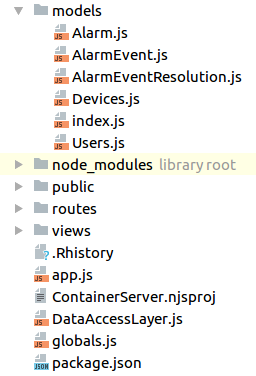
\includegraphics[scale=0.6]{gfx/structure}
\end{figure}
\smallskip

The overall structure can be seen on a following class diagram (please note that due to nature of node.js and reccommended practices for sequelize.js and express.js the OOP paradigm was not fully applied and hence the class diagram is bolted onto based on the file names and functions they define):
\bigskip
\begin{figure}[H]
\centering
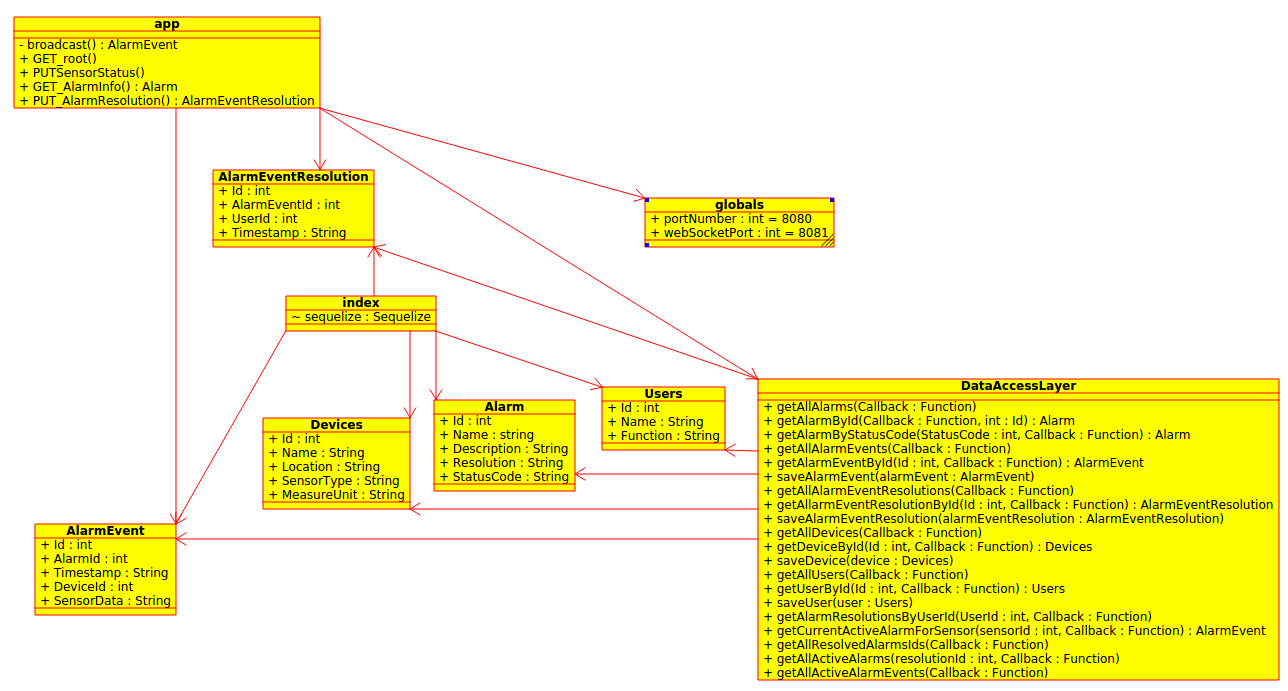
\includegraphics[scale=0.3]{gfx/class}
\end{figure}
\smallskip
As a short explanation to the class diagram above it is important to point out that the index.js file is picked up by sequelize at execution and hence it is not imported within any of the other files explicitely.

\smallskip

One final thing worth mentioning is presence of database deployment script that creates and initializes the database automatically. The script is an SQL Script with executor implemented as both bash and batch script hence it is possible to be executed on multiple environments. The script is present in the DBScripts folder in the root folder of the repository.
%%% Local Variables:
%%% mode: latex
%%% TeX-master: "../ClassicThesis"
%%% End:

\section {BLE node}
\label {Impl_BLEnodeSection}

The sensing node is supposed to be installed on the container. For the demonstration purposes, we used a Raspberry Pi 3 device running NodeJs.

The BLE node has a DHT22 sensor that is able to sense temperature and humidity. The following diagram shows the wiring setup between the Raspberry device and the sensor. The sensor has 3 pin connections - 2 of them being used for power (VCC and ground) while the third is for transferring data. The a compatible driver for this sensor is required to be installed on the node.

\bigskip
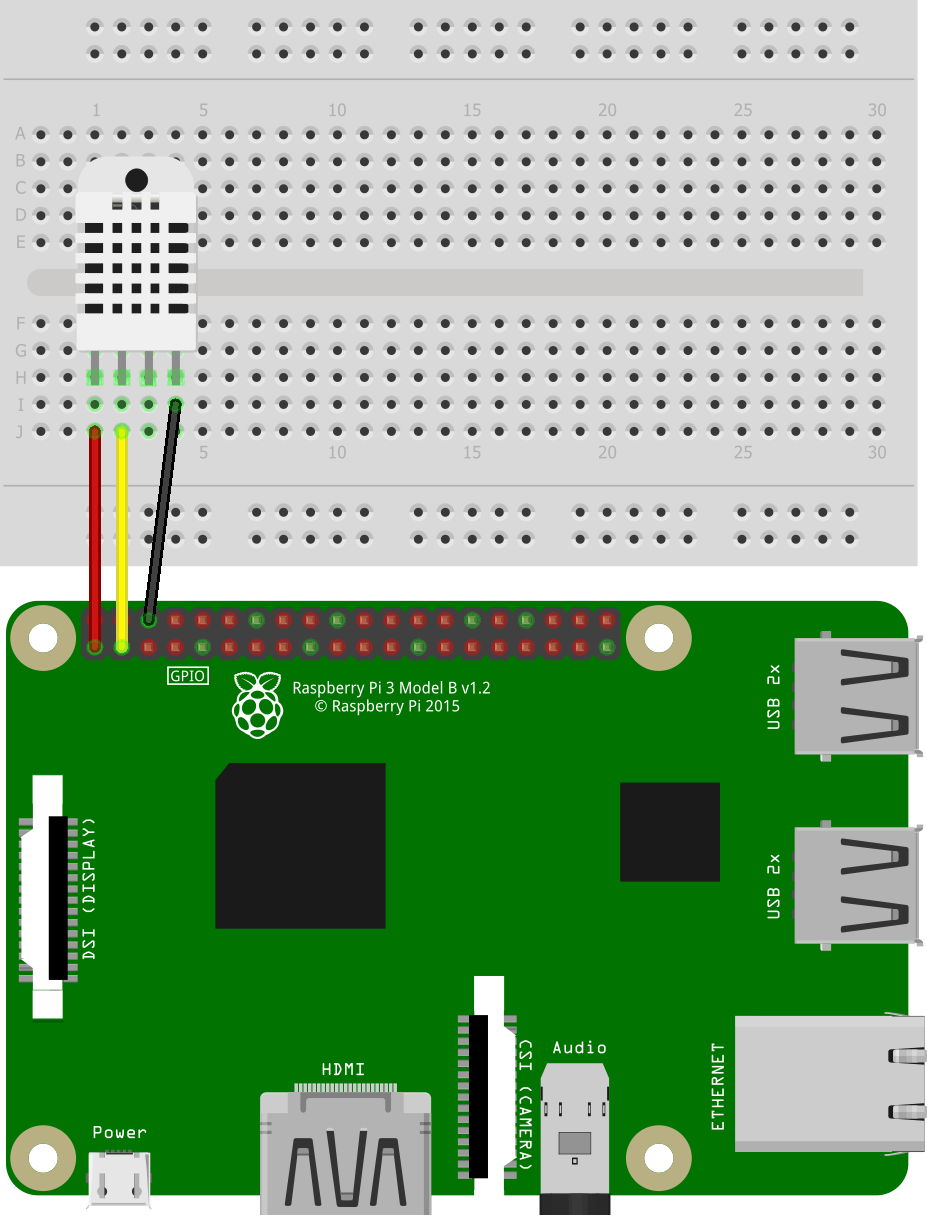
\includegraphics[scale=0.7]{gfx/RaspberrySensorNode} 
\bigskip

To interface with the sensor from the Node application, a npm package called node-dht-sensor needed to be added to the project.

The Nodejs application for the BLE node is structured as shown in the following diagram. For each of the components, the most important public methods are shown in order to show the interfacing between them. Private methods and members are not included to maintain the simplicity of the diagram.

\bigskip
\includegraphics[scale=0.6]{gfx/bleNode_Architecture} 
\bigskip

For each file, a short description of its purpose is provided.
\begin{itemize}
\item bleAdvertiser - class used for handling the BLE broadcasting. The sensor id and status code are broadcasted as the name of the device, separated by a semi-column. As the maximum name size allowed is 31 bytes, this field is more than enough for the information we require to make public. The class has only one public method that takes as argument the status code to broadcast.
\item restClient - class incorporating the logic and callbacks for making rest API calls over the network. This class exposes one public method used by the application to report the status and sensor data to the main server.
\item sensorInterface - class constantly pooling the data from the sensor and providing it when needed to the main application logic. This class is using an internal timer to control the frequency of poling sensor data.
\item utils - class containing helper methods used by the other components in the application. In this class, one method for comparing two different instances of sensor data in json format is provided. This is required to prevent the node from sending redundant data to the main server.
\item app - this is the main class of the application. It incorporates the rules and conditions for determining the status codes and uses most of the other classes, each having a specific role.
\item globals - class used for holding a set of global variables used throughout the application. The containing json file can therefore be used as application configuration that has different contents depending on the deployment sensor nodes.
\end{itemize}

The BLE node is designed to call only one REST method on the main server - reportStatus. This has been however thought so the sensor can both report data and aliveness. The sensor therefore calls the method each time the data or sensor status changes. If the measured values are constant, a call will be made every minute. This ensures that the time interval between 2 sensor updates is 60 seconds or less. Using this approach allows the server to determine whether the sensor is no longer active/connected to the network and inform the users accordingly. 




\section {Android node}
\label {Impl_AndroidNodeSection}

Write here...



%%% Local Variables:
%%% mode: latex
%%% TeX-master: "../ClassicThesis"
%%% End:
